\section{Overall Description}

%  in automatico Section [number]
\subsection{Product
perspective}
Here we discuss in details all the shared phenomena outlined in Section 1.3 and we also provide a domain model through class and state diagrams.
\\\newline
    \noindent\textbf{Shared Phenomena, controlled by the world and observed by the machine. }
\begin{itemize}
    \item Register/login: a normal person or a municipality worker can register to the application through two different intuitive forms; SafeStreets collects all the information inserted by the User, creates an account and verify the validity of the information given through a email-confirmation message. Once the User confirms its account he/she can proceed to login.
    \item Report of a traffic violation: the User is able to report traffic violations at any time, he/she can open the application, select \textit{take a picture} and then send the report including the picture, the type of violation and the name of the street where the violation occurred.
    %levato perché forse non ha senso
    %\item Addition of further information: the User can add further information to the report that is going to be sent, the information can be the license plate of the car, the exact street in which the car was parked, the time in which
    \item The Municipality offers up-to-date information about accidents: in the Municipality web platform there is a service (daily updated) that indicates streets in which accidents occurred. In this way the System can observe safe/unsafe areas.
\end{itemize}

    \noindent\textbf{Shared Phenomena, controlled by the machine and observed by the world.}
      \begin{itemize}
      % controllare se forwarding va bene
          \item Forwarding of traffic violations: every time a user sends a traffic violation, the System forwards it to the authorities. The message sent by the System contains the photo of the violation, the type of violation, the street in which it took place and the area in which the photo was taken (since there may be more than one street with that name).
          \item Visualization of own reports: the System makes it possible for the users to view the own reports by performing a query to the database and displaying them in a ListView in the application.
          %forse no?
          %\item Verification of identity of the User:
          \item Visualization safe/unsafe areas: the System through the service offered by the municipality is able to get a list of areas in which accidents took place, thus the System can show unsafe and safe areas to the User.
          % c'è una parola per una cosa che avviene spesso, ma non me la ricordo, se ve la ricordate fatemi sapere per favore. grazies.
          \item Suggest possible interventions: the System,  by using a list of known and effective solutions for some common violations, is able to suggest possible interventions in order to reduce the number of violations and make unsafe areas safer.
          % poi safer non mi piace tantissimo
          \item Generate traffic tickets: the municipality, by observing the reports provided by Safe4Streets, is able to  generate traffic tickets by using a functionality of the application.
          % forse non ci va funcionality ma opzione
          \item Notify about modified photos: if the User modifies a photo in order to send malicious reports, the system mark the User as a malicious User and sends a message about this event to authorities (that already received reports created by the User). 
          % mi ricordavo che to illustrate è bello da dire
          \item Generate statistics: the System is able to generate graphs that illustrate statistics, like the most egregious offenders, the effectiveness of the application itself, etc.
          \end{itemize}
          

\vspace{40px}      

\subsubsection{Class Diagram}
    \begin{figure}[h]
        \centering
        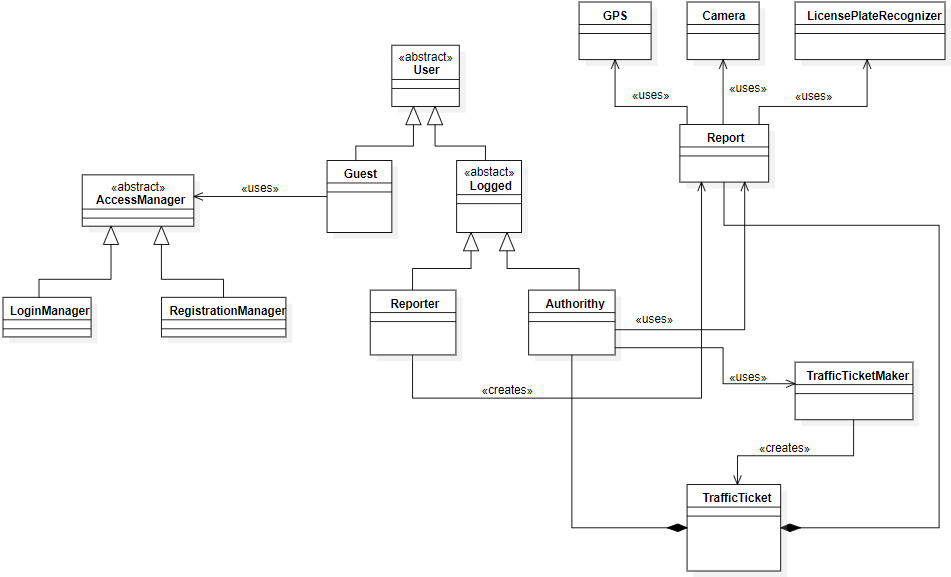
\includegraphics[scale=0.5]{Images/ClassDiag.png}
        \caption{Class Diagram}
    \end{figure}

\newpage

\subsubsection{State Diagrams}
    \begin{figure}[h]
        \centering
        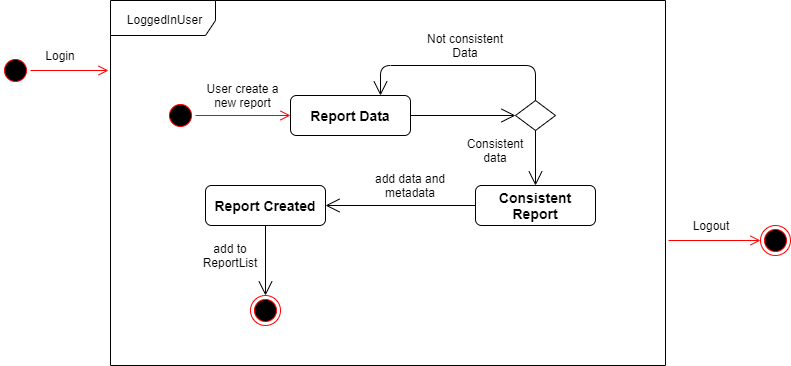
\includegraphics[scale=0.5]{Images/StateDiag_addReport.png}
        \caption{State Diagram of the insertion of a new Report by an User}
    \end{figure}
    
    \vspace{30px}
    
    \begin{figure}[h!]
        \centering
        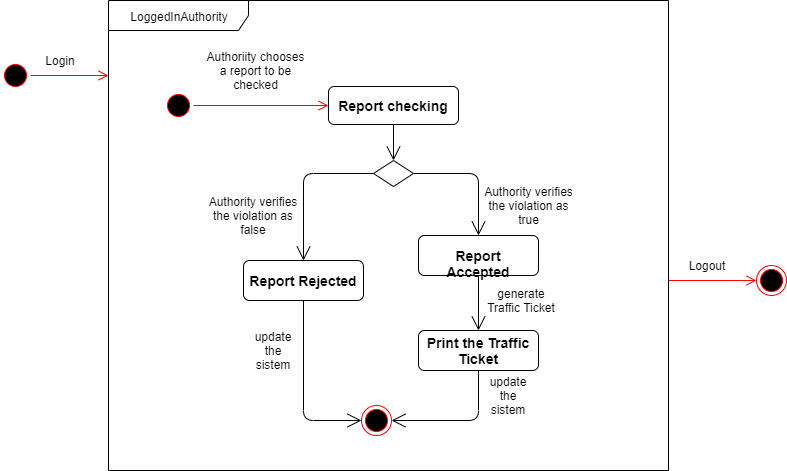
\includegraphics[scale=0.5]{Images/StateDiag_verifyReport.png}
        \caption{State Diagram of the checking of a Report by an Authority}
    \end{figure}


\subsection{Product
functions}

\textbf{SafeStreets}\\

\textit{SafeStreets} was born with the intention of improving urban traffic mobility, by collecting notifies made by Users about many kinds of traffic violations. Then these information can be consulted by Users themselves, or from a Third Part, the traffic competent authorities, or the municipality, which can create tickets based on these information, on which integrity it is necessary to pay particular attention. Indeed, \textit{SafeStreets} provides useful suggestions built upon the crossing of municipality's and \textit{SafeStreets}'s data. \\
Let's see more in the details the functions mentioned above:\\\\

\textbf{Basic User functions} \\
\begin{itemize}
    \item \textbf{Notifying violations}\\\\
    The Users who is witness of a rule violation, and wants to notify it through \textit{SafeStreets}, has to be registered to the application; then he/she can fill up the notification form provided by the application, with a picture or a video of the violation occurring, the kind of violation, the kind of vehicle, the position, (or the address, which can be anyway gathered from GPS), and the license plate of the indeed vehicles.\\
    Not all of these data are mandatory for the User to send, only a picture, the GPS position and the kind of violations are: \textit{SafeStreets} uses an algorithm to catch the license plates from the picture, can obtain the address by the GPS position, and it implements a deep learning algorithm to recognize the vehicles by it self. \textit{SafeStreets} is going to attach these computed metadata to the notification, in case of missing. Time is automatically taken from the notification delivery time.
    
    \item\textbf{Mining information from data}\\\\
    Users can access the  data stored by the application, in order to mine useful information. \\ \textit{SafeStreets} provides an easy-use interface that allows to  carry out a search for violations based upon different criteria: the \textit{kind} of the violations, the \textit{place} in which happen, the \textit{time}, and the \textit{kind of vehicle} involved. 
    A user can then extract information from this data, for example, search for a place, and then see at which time slot of the day, more violations are committed in that place, or in which place or at which time slot, a precise type of violation occurs the most.\\
    By the way, due to privacy purposes, license plates related to violations are not visible by a normal User, neither a User can search some information about a precise vehicle with a precise license place.
    
    \end{itemize}  
    
    \textbf{Authority Users functions} \\
    
    \begin{itemize}
   
    
    \item\textbf{SafeStreets suggestion mechanism}\\\\
    If the local municipality provides a way to access their own urban traffic and violations data, \textit{SafeStreets} can cross them, to enlarge the amount of information accessible, and exploit them to formulate suggestions for the municipality, in order to increase the functionality of the urban infrastructure, reduce the violations, improve road conditions.\\ Authorities and municipality can ask for these suggestions for various areas, with a function button on the application interface.\\
    Imagine a situation in which \textit{SafeStreets} knows about huge amount of bike lane invasion violations, and municipality knows that in that zone, many people use bikes for moving, then \textit{SafeStreets} can cross those information and provide the suggestion to build a separation line between the car road, and the bike lane, because it should be a good investment, knowing the fact that not only there are lots of violations, but also that those could be very dangerous, given the number of people using bike in that zone. 
    
    
     
    \item\textbf{Searching for violations}\\\\
    In addition to the mining functions provided for normal users, Authorities can also access some more "sensible data", and carry out more precise searches about violations. They can access the list of violations, with relatives license plates and data of involved people. In order to build this authorization diversification, a different type of registration will be reserved for authorities Users. (Da decidere come).
    Authorities can also use the application to get suggestions about which are the most unsafe urban areas, and how to get them better.
    
    
    \item\textbf{Traffic tickets service}\\\\
    \textit{SafeStreets} give road Authorities the possibility to generates traffic tickets from the violations information sent by Users. An appointee authority User can check a notified violation and all the data attached to it, confirm that it is actually a violation, and then the use function provided by \textit{SafeStreets} (that is linked to the authorities management system) to generate a ticket. \\
    In order to make this right, \textit{SafeStreets} has to ensure that the chain of custody of the data, from the user to the data store, is completely reliable. To do this, security algorithms perform a validity check on the sent pictures, to be sure the picture is not been modified. In case it is, discard the notification. Discarded data are used to make statistical analysis.
    Another filtering level is applied by allowing Users to only send pictures taken while filling up the notification form, and not to upload previously taken ones. In this way, it's harder for a User to modify a picture before sending it. 
\end{itemize}

\subsection{User
characteristics}
% se non vi piace possesses pssiamo cambiarlo
SafeStreets is an application suitable for any adult person that possesses a mobile phone.
\subsubsection{Actors}
\begin{itemize}
    \item \textbf{Guest}: a person who downloaded the application and still has to register, he cannot use any functionality of the application.
    \item \textbf{User}: once a guest has registered through the initial form of the application, he gets an account with a \textit{username} and a \textit{password}. Moreover, the User has accepted to give his location and access to the camera of the mobile phone.
    \item \textbf{Authority}: a municipality worker that is able to generate traffic tickets from the violations reported. Furthermore, he can access to other functionalities that a simple user cannot even see.
    %non mi viene in mente nessun altro
    %\item \textbf{}
\end{itemize}
\subsection{Assumptions,
dependencies
and
constraints}


\subsubsection{Domain Assumptions}
\begin{itemize}
    \item {[D.1]} Personal data given by Users during the registration process are assumed to be correct.
    %\item {[D.2]} Each User is assumed to be unique.
    \item {[D.3]} Pictures sent by Users are assumed to be in some precise file format.
    \item {[D.4]} The GPS is assumed to be subject to some precision error.
    \item {[D.5]} Violations for which a ticket is generated are supposed to be validated by authorities first.
    \item {[D.6]} Information obtained by authorities are supposed to be correct.
    \item {[D.7]} Is assumed that there's no bounds which suggestions provided by the S2B have to respect.\\
\end{itemize}

\subsubsection{Dependencies}
\begin{itemize}
    \item The S2B will use the GPS service of the Users smartphone.
    \item The S2B will use the camera function of the Users smartphone.
    \item The S2B will use the internet connectivity of the Users smartphone.
    \item The S2B will rely on a DBMS to store all the obtained data.
    \item The S2B will use some external API to provide  a map view service to the Users.
    \item The S2B will use the information provided by local municipality, to cross data and create suggestions.\\
\end{itemize}


%\subsubsection{Constraints}




